% !TEX TS-program = pdflatex
% !TEX encoding = UTF-8 Unicode

% This is a simple template for a LaTeX document using the "article" class.
% See "book", "report", "letter" for other types of document.

\documentclass[11pt]{article} % use larger type; default would be 10pt


\usepackage{ulem}
\newcommand\NoIndent[1]{%
  \par\vbox{\parbox[t]{\linewidth}{#1}}%
}


\usepackage[utf8]{inputenc} % set input encoding (not needed with XeLaTeX)

%%% Examples of Article customizations
% These packages are optional, depending whether you want the features they provide.
% See the LaTeX Companion or other references for full information.

%%% PAGE DIMENSIONS
\usepackage{geometry} % to change the page dimensions
\geometry{a4paper} % or letterpaper (US) or a5paper or....
% \geometry{margin=2in} % for example, change the margins to 2 inches all round
% \geometry{landscape} % set up the page for landscape
%   read geometry.pdf for detailed page layout information

\usepackage{graphicx} % support the \includegraphics command and options

% \usepackage[parfill]{parskip} % Activate to begin paragraphs with an empty line rather than an indent

%%% PACKAGES
\usepackage{booktabs} % for much better looking tables
\usepackage{array} % for better arrays (eg matrices) in maths
\usepackage{paralist} % very flexible & customisable lists (eg. enumerate/itemize, etc.)
\usepackage{verbatim} % adds environment for commenting out blocks of text & for better verbatim
\usepackage{subfig} % make it possible to include more than one captioned figure/table in a single float
% These packages are all incorporated in the memoir class to one degree or another...

%%% HEADERS & FOOTERS
\usepackage{fancyhdr} % This should be set AFTER setting up the page geometry
\pagestyle{fancy} % options: empty , plain , fancy
\renewcommand{\headrulewidth}{0pt} % customise the layout...
\lhead{}\chead{}\rhead{}
\lfoot{}\cfoot{\thepage}\rfoot{}

%%% SECTION TITLE APPEARANCE
\usepackage{sectsty}
\allsectionsfont{\sffamily\mdseries\upshape} % (See the fntguide.pdf for font help)
% (This matches ConTeXt defaults)

%%% ToC (table of contents) APPEARANCE
\usepackage[nottoc,notlof,notlot]{tocbibind} % Put the bibliography in the ToC
\usepackage[titles,subfigure]{tocloft} % Alter the style of the Table of Contents
\renewcommand{\cftsecfont}{\rmfamily\mdseries\upshape}
\renewcommand{\cftsecpagefont}{\rmfamily\mdseries\upshape} % No bold!

%%% END Article customizations


\usepackage{verbatim}
\usepackage{amsmath}


\title{Work Log for September}
\author{Logan Brown}
%\date{} % Activate to display a given date or no date (if empty),
         % otherwise the current date is printed 

\begin{document}
\maketitle

FOREWORD: I think for October, I'll just do the monthly summary. The things I'm doing are now carrying over well from week to week.

\tableofcontents

\newpage


\setcounter{section}{0} %week number minus 1
\setcounter{subsection}{-1}
\setcounter{subsubsection}{0}

\section{Week of September 1st-5th}
\subsection{Goals for the Week}
\begin{enumerate}
\item Connect codons with $\Delta$eta values
\item Liz Howell Code
\item Further readings in the R user manual
\item NSE Model
\end{enumerate}

\subsection{Progress/Notes}

\subsubsection{Connect codons with delta eta values}
I made a change to run\_roc.r, line 314. I changed

\noindent mean.b.mat $<$- cbind(bmat.names, mean.b.mat, sd.b.mat)

	to
	
\noindent mean.b.mat $<$- cbind(names(results\$chains[[1]]\$b.Mat[[1]]), mean.b.mat, sd.b.mat)

bmat.names is just the synonym group of the codon. names(results\$chains[[1]]\$b.Mat[[1]]) is of the format aminoacid.codon.value (for example A.GCC.log.mu or H.CAC.Delta.t where log.mu represents the natural log of the mutation rate and Delta.t represents the change in the pausing times (compared to some reference codon). This information gets written to 

A note on the reference codon: Cedric claimed the one with the shortest pausing time was the reference codon, I've found it's the last one alphabetically.



\subsubsection{Liz Howell Code}
The code seems to be done. It can be checked out from github at

https://github.com/ozway/optimal-pessimal.git

It takes in a gene (by default, named "ecoli.fasta"), and can write the optimal or pessimal version(s) of the genome using makeOptimal.r, makePessimal.r, or makeBoth.r. The optimal is written to optimalEcoli.fasta, and the pessimal is written to pessimalEcoli.fasta. writeOptimal and writePessimal takes about 5 minutes and 49 seconds to run on the ecoli gene. writeBoth takes about 7 minutes and 45 seconds to run on the ecoli gene, likely due to the increased file writing.

~

\noindent Future Considerations:
\begin{enumerate}
\item \sout(Add a config.r file for setting global variables like input filenames and output filenames) Done
\item Calculate the total amount of time gained or lost in the changes
\item Do we need to switch from ROC to $\eta$?
\item Try for other genes?
\end{enumerate}

I've also written up readme instructions for how to execute the code.


\subsubsection{Further readings in the R user manual}
In order to write the Liz Howell code, I had to do more readings into the R user manual. I read deeply into, and played around with
\begin{itemize}
\item Matrices
\item Lists
\item String Manipulation
\item the [] and [[]] operators
\item for and while loops
\end{itemize}

\subsubsection{NSE Model}
Following Wei-Chen's instructions, I attempted to run a cubfits NSE model.
\begin{enumerate}
\item Change the cubmultichain and cubsinglechain calls on lines 188, 195, 205, 212, changing model=``roc" to model=``nsef"
\item Before each of those lines, add .CF.CT\$model $<$- ``nsef";
\end{enumerate}
And then running it as normal.


9/5: I started the model at at 9:02. After generating very little output, it ended at 12:38. It parsed all the inputs and such, but generated no results.


\section{Week of September 8th-15th}
\subsection{Goals for the Week}
%Paste output from writeGoals

\begin{enumerate}
\item NSE Model

\end{enumerate}

\subsection{Progress/Notes}

\subsubsection{NSE Model -- run using workflow.sh}
These are the changes I've made to cubfits/misc to try and run the NSE model. (run\_nsef.r is just a copied version of run\_roc.r with the following exceptions)
\begin{itemize}
\item In run\_nsef.r, changed model=``roc" to model=``nsef" in cubsinglechain and cubmultichain for both "cubfits" and "cubappr"
\item In run\_nsef.r, added .CF.CT\$model $<$- "nsef"; before each each call of cubsinglechain and cubmultichain
\item In run\_utility.r, changed get.logL $<$- function(ret, data, model="roc") to get.logL $<$- function(ret, data, model="nsef")
\item Changed workflow.r from 
\begin{itemize}
\item Rscript run\_roc.r -c \$cubmethod -s "0.5 1 2 4" -f \$genome -p \$empphi -o \$folder -n \$foutname -i \$pinit $>>$ \$logfile \& 

to

\item Rscript run\_nsef.r -c \$cubmethod -s "0.5 1 2 4" -f \$genome -p \$empphi -o \$folder -n \$foutname -i \$pinit $>>$ \$logfile \&
\end{itemize}
\end{itemize}

I also changed to cubsinglechain instead of cubmultichain, to try and simplify matters, but then the MCMC started throwing "acceptance out of range" at every step of the iteration. Started at 10:44, ran until 11:44. 

I'll retry with cubmultichain. I had run a multichain version on 9/5, and it just stalled. However, I just added run\_utility.r change

Latest settings that worked!
\\n.samples = 10  
\\use.n.samples = 10
\\n.chains = 4
\\n.cores = 4
\\min.samples=50
\\max.samples=100

\verbatiminput{data/sep8.nse.100samples.log}


I was able to repeat these results using 1000 samples, (minimum of 500 samples), though it stopped after 500 samples. The Gelman score was 1.10581040617552. For brevity, the 500 sample log is not included in this pdf, but it is in the github.


\subsubsection{Larger NSE Model}

Ran from 17:22 to 19:12, then ended with no error messages. "Timing stopped at"

Is it possible that the model is OVERconverging? I had it doing 500 samples between checks, and it should succeed at doing 500 samples...


\subsubsection{NSE Model -- debug}

Ran the contents of cubfits/demo/nsef.train.r in an R interactive session, adding in the line debugonce(cubfits)

As far as I can tell, the cubfits() function itself doesn't actually use the model or .CF.CT\$model, I'll need ot look at drawP and drawPhi.

According to Cedric, it's worthwhile to look at cubfits/cubfits/R/my.logdmultinomCodOne.r. That function calls cubfits/cubfits/src/stable\_exp.c and cubfits/cubfits/src/lib.c.


\subsubsection{Optimal/Pessimal Code}

Cedric made the change that had been discussed, where we switch from $\Delta t$ values to $\Delta\eta$

In making that change, I also made several more changes.

\begin{itemize}
\item fixed a bug where the default codon for Q was wrong
\item Changed from analyzing $\Delta t$ to $\Delta\eta$ values. Made a mock up etaValues.bmat for example by just inverting the signs of the values
\item made the language more clear for "optimal/best" versus "minimum/maximum"
\item added a count and ratio for how many codons are actually being up/downgraded
\end{itemize}

Deepika contacted me about an error in the code. The beginning of the for loop (line 78 in the original, now line 79)

for(index in 1:length(sequence[[gene]]/3))\{
\\to

for(index in 1:(length(sequence[[gene]])/3))\{

~

The first one was causing a fractional value of index, which was making it do weird things, but mainly, it was making the code replace random chunks of genome, rather than accurately dividing the codon into groups of 3.


\subsubsection{First Order Approximations}

For completeness, I also wrote down how we derived the fitness function in fitnessHistory.tex


$p_{ic}$ is the probability of a nonsense error at position $i$ using codon $c$
\\ $p_j$ is the probability of a nonsense error at position $j$

~

First order approximation about $p_{ic} = 0$ is
$$f(p_{ic} \approx f(0) + f'(0)*(p_{ic}-0)
= p_{ic}\left(
\left[\sum_{k=1}^{i} a_1 + a_2(k-1)\right]
\left[\prod_{j=i+1}^{n}(\frac{1}{1-p_{j}})\right]
\right)
$$


First order approximation about $p_{i+1} \approx p_{i+2} \cdots \approx p_{n} \approx 0$ is

$$
f(p_j) \approx
\left[\sum_{k=1}^{i} a_1 + a_2(k-1)\right]
\left[\frac{p_{ic}}{1-p_{ic}}\right]
+
\left( (i+1) - n \right)
\left[\sum_{k=1}^{i} a_1 + a_2(k-1)\right]
\left[\frac{p_{ic}}{1-p_{ic}}\right]
\left( p_{j} \right)
$$

$$
f(p_j) \approx
f(0) + (f(0))(p_j)((i+1)-n)
$$


Details are in approx.tex


\subsubsection{Simulated Data Set from REU13}
The data is in /home/lbrown/reucode/data/inputsimdata/REU\_data

I think elongation rate refers to the odds $\frac{p_i}{1-p_i}$.



\subsection{Goals for next Week}
\begin{enumerate}
\item Simulated Data Set
\item Potentially look at the c files in cubfits/cubfits/src
\item \sout{Code the first order approximations? Looking at my draw*.r for the fitness function}
\item Check for problems in Wei-Chen's NSE code, specifically
\begin{enumerate}
\item \sout{Unnecessary VGLM calls leading to longer run times} As far as I can tell, my.fitMultinomOne.nsef and my.fitMultinomOne.roc are using the same amount of vglm calls.
\item Ending crash caused by running out of memory
\end{enumerate}

\item Continue to improve the optimal-pessimal code as Deepika works with it.
\end{enumerate}


\section{Week of September 15th-19th}
\subsection{Goals for the Week}
%Paste output from writeGoals
\begin{enumerate}
\item Simulated Data Set
\item cubappr SimuYeast Run
\item First Order Approximation
\item Potentially look at the c files in cubfits/cubfits/src
\item Investigate WeiChen NSE crash
\item Compare NSE code to ROC code
\item Build Local Cubfits
\item Disect NSE data Structure
\item Profile the ROC model (where is the time?)
\item Profile the NSE model if possible
\item Continue to improve the optimal-pessimal code as Deepika works with it.
\end{enumerate}

\subsection{Progress/Notes}

\subsubsection{Simulated Data Set}
The data is in /home/lbrown/reucode/data/inputsimdata/REU\_data

As I understand it, these fasta genomes are ones that have been modified by Codon Evolution Simulation (CES). A quick comparison of  b-1/S.cerevisiae.S288c.REU.sim.b-1.ces.fasta and ../S.cerevisiae.S288c.fasta shows that they have different codons. Additionally b-1's fasta file and b-0.01's fasta are different as well.

The folder b-1 vs b-0.1, etc is the setting of the B parameter. Look at '/export/home/clandere/CodonUsageBias/NSE/ces3/branches/exchange/C/data\_simulation/CES.DATA.SIM.README.pdf' for more details

I chose to use b-0.001, it had the best signs of actually converging to something. The eta values of the genes actually changed. For some b values, there wasn't an eta change. b-0.001/S.cerevisiae.S288c.REU.sim.b-0.001.evol.summary.tsv was the highest B value that had changes at every genome (Evolution Time != nan). 

I was not able to find X\_obs values for the yeast data in the REU data. I found ORF data in /opt/big\_scratch/work-my, which is data from Wei-Chen/Yassour. I ran a recursive search through those files looking for xobs values, the output is found in smallfindXobs.txt



\subsubsection{cubappr SimuYeast Run}
Launched a cubappr run of the simulated yeast genome from the REU data, both for single chain and \sout{multichain} (nothing happened for ~2 hours. either it crashed, or changing the config.r file messed with the actual inner workings). If either/both crashes, I'll try again with a smaller run, likely just singlechain.


\subsubsection{First Order Approximation}

$$\prod_{j=i+1}^{n} (1-p_j)= \prod_{j=i+2}^{n} - p_{i+1}\left(\prod_{j=i+2}^{n}(1-p_{i+1})\right)$$

Simply to make things easier to read, I'll restate $\prod_{j=q}^{n} (1-p_j)$ as $t_q$. Note that in general,

$$t_q = t_{q+1} - p_q(t_{q+1})$$

So 

\begin{align*}
	\prod_{j=i+1}^{n} (1-p_j) &= t_{i+2} - p_{i+1}t_{i+2} \\
	&= t_{i+3} - p_{i+2}t_{i+3} - p_{i+1}\left(t_{i+3} - p_{i+2}t_{i+3}\right) \\
	&= t_{i+3} - p_{i+2}t_{i+3} - p_{i+1}t_{i+3} - p_{i+1}p_{i+2}t_{i+3}
\end{align*}

Since $p_{i+1} * p_{i+2} \approx 0$.

$$\approx t_{i+3} - p_{i+2}t_{i+3} - p_{i+1}t_{i+3}$$

Continuing iteratively...

\begin{align*}
	\prod_{j=i+1}^{n} (1-p_j) &\approx
	t_n - \sum_{k=i+1}^{n-1}p_k(t_n) \\
	&\approx (1-p_n) - \sum_{k=i+1}^{n-1}p_k(1 - p_n)\\
 	&\approx 1 -  \sum_{k=i+1}^{n}p_k
\end{align*}

\subsubsection{Potentially look at the c files in cubfits/cubfits/src}
They take up the majority of the time (see the profiling below)

lp\_c\_raw


\subsubsection{Investigate WeiChen NSE crash}
\begin{itemize}
\item Ending crash caused by running out of memory?
\end{itemize}

Cedric also suggests it could be due to a problem with the serialization step. When the code is run in parallel (by SNOW activating multiple copies of the same program with different initial conditions), it comes back to the serial to be tested for convergence. If the data structures are too large at this point, it may crash due to "running out of memory", even though Gauley has waaay more memory. It may be related to memory.c

I'm running in single chain from here on out for testing this hypothesis.

Single chain crashed, however, it actually told the error!

\verbatiminput{data/sep15.SimYeastNSE.error.txt}

\subsubsection{Compare NSE code to ROC code}

Here are all the files that use the NSE model (results of grep -il nse ~/cubfits/cubfits/R/*)


\sout{my.coef.r}\\

my.estimatePhiOne.r\\
my.fitMultinomOne.r

Here is where the vglm concerns are. Mostly not concerned, it doesn't look like any additional vglm calls.\\


my.logdmultinomCodOne.r\\

Here's my biggest concern. 


my.logdmultinomCodOne.roc has three lines that my.logdmultinomCodOne.nsef does not
  lp.c.raw $<$- yaa * lp.vec
  lp.c.raw[is.nan(lp.c.raw)] $<$- NA
  lp.c.raw $<$- rowSums(yaa * lp.vec, na.rm = TRUE)

my.drawPhiConditionalAllPred calls my.logPosteriorAllPred.lognormal, which calls my.logdmultinomCodOne.nsef, which does not have the stated lines. Without those lines, if lpProp - lpCurr - prop\$lir becomes NaN (log of a negative value, most likely), it would not pass any errors until the line that actually complains, accept $<$- u $<$ exp(logAcceptProb).

However logAcceptProb is lpProp - lpCurr - prop\$lir

My best hypothesis is that lpProp (proposed phi values from the Posterior distribution) has some NaN values.


CONFIRMED, 

\verbatiminput{data/sep19.nse.lpPropisNaN.tail}

lpProp is coming up with NaN. I suspect that negative phi values are being proposed, and $ln(-x)$ is NaN, and $e^{NaN}$ is NaN, etc, etc, etc, NAs are not allowed in subscripted assignments.

I'll add browser() lines to my.logdmultinomCodOne.r and see what happens. I also removed the \& from the end of the line to be sure the browser command will work.


~


Probably don't need to be considered, but left here for completeness

~\\
my.objectivePhiOne.Lfp.r\\
my.objectivePhiOne.nlogL.r\\
my.objectivePhiOne.nlogphiL.r\\
my.objectivePhiOne.phiLfp.r\\
my.pPropTypeNoObs.lognormal\_bias.r\\
plotbin.r\\
plotmodel.r\\
simu.orf.r\\


\subsubsection{Build Local Cubfits}

\begin{enumerate}
\item cd path/to/cubfits/..
\item R CMD build cubfits (This creates cubfits\_ver.si-on.tar.gz)
\item R
\item install.package("\_\_\_\_\_\_\_.tar.gz", lib ="place to install to", repos = NULL, type="source")
\item library(cubfits, lib.loc="place you installed to")
\end{enumerate}


\subsubsection{Disect NSE data Structure}

\subsubsection{Profile the ROC model (where is the time?)}
Look at the man page - ?Rprof 

%Rprof(filename = "Rprof.out", memory.profiling = TRUE);
Run Rprof() before any code you want to profile, and Rprof(NULL) after the code, then run summaryRprof in R or R CMD Rprof from the command line to analyze the output. 

Added Rprof() to the beginning of run\_roc.r and Rprof(NULL) to the end of run\_roc.r, then ran using ./workflow as usual.

These are the functions that took up more than 1\% of the time on their own.
\verbatiminput{data/ROC_Profile1percent}

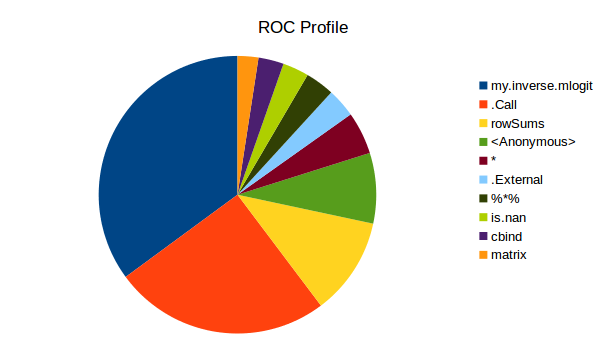
\includegraphics{data/ROC_Profile}
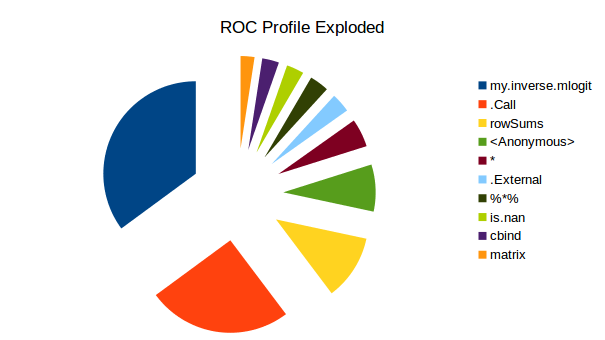
\includegraphics{data/ROC_Profilexplode}

.Call is only seen in two places\\
.Call("invmlogit"... in my.inverse.mlogit.r\\
.Call("lp\_c\_raw"... in my.logdmultinomCodOne.r

It's the function that calls the C code from the R code. The C code, apparently, is doing the bulk of the work.


\subsubsection{Profile the NSE model if possible}

I ran an incomplete run of the NSE model, crashing in the usual place, but profiled it.

\verbatiminput{data/NSE_IncompleteProfile1percent}

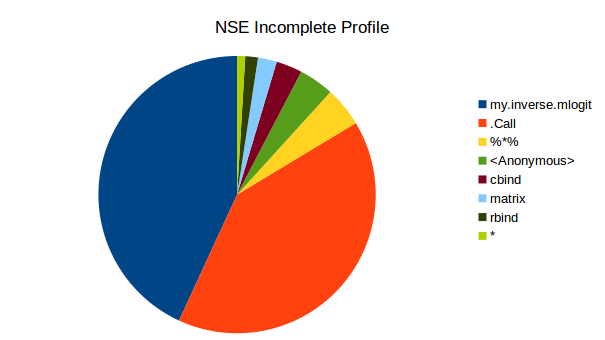
\includegraphics{data/NSE_IncompleteProfile}
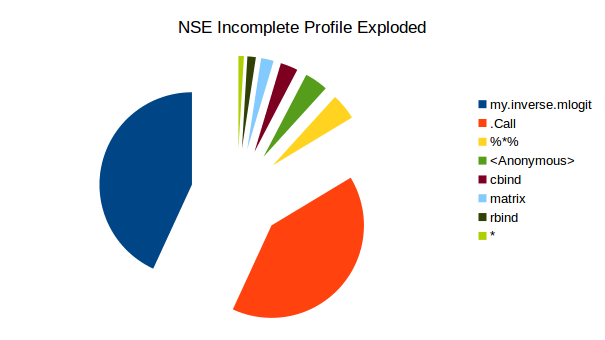
\includegraphics{data/NSE_IncompleteProfilexplode}



\subsubsection{Continue to improve the optimal-pessimal code as Deepika works with it.}





\subsection{Goals for next Week}
\begin{enumerate}
\item Write out the math from 9/19 (from the green notebook)
\item Run NSE model with the Browser line when $phi$ is proposed to see what is causing NaN
\item Ideally, an NSE patch to fix it (try NaN to NA?)
\end{enumerate}


\section{Week of September 22nd-26th}
\subsection{Goals for the Week}
\begin{enumerate}
\item Write out the math from 9/19 (from the green notebook)
\item Get observed yeast phi values from REU data
\item Run NSE model with the Browser line when $phi$ is proposed to see what is causing NaN
\item Ideally, an NSE patch to fix it (try NaN to NA?)
\item Disect NSE data structure
\end{enumerate}

\subsection{Progress/Notes}

\subsubsection{Write out the math from 9/19 (from the green notebook)}

see genomeProb.tex and genomeProb.pdf

\subsubsection{Get observed yeast phi values from REU data}

\subsubsection{Run NSE model with the Browser line when $phi$ is proposed to see what is causing NaN}

7/22: The local library has been built. I removed the \& to ensure that browser() will activate, and and wrote in two checks in my.logdmultinomCodOne.r

\verbatiminput{misc/browsercommand.txt}

but it's taken nearly 8 hours to run!!! The run started at: 2014-09-22 10:24:55 

I left at 18:15:, so I don't know what happens.

The run finished at 18:28. But... browser didn't launch? I think I'll have to go into R manually, and use

\verbatiminput{misc/browsercommand2.txt}

This means I'll have to parse the command line arguments manually.


CAUGHT

\verbatiminput{misc/errorlogs.txt}

This means that it's actually not catching in my.logdmultinomCodOne.r

It catches in my.drawPhiConditionalAll. \sout{but lpProp comes from my.logPosteriorAll.lognormal\_bias. Which comes from} .cubfitsEnv does not correctly get MY functions. So it never got my.lodgmultinomCodOne with the browser() commands. Interesting.

I've done two separate runs of nsef cubfits.

\begin{enumerate}
\item one of the elements of lpProp is going to NaN.
\item It is not always the same element. For my first run, it was zraS. The second was ecnA.
\item It is not because log(0)$= -\infty$. Multiple elements are going to -Inf (106 in the first run,  87 in the second run). Moreover, the roc code also tends to generate -Inf values (though not nearly as many in each run, only 1 or 2).
\item It doesn't appear that the scale is going out of control. Scale and acceptance rate stay similar to the values used in the ROC model.
\item It happens in cubfits and cubappr 
\item It is not just happening for one amino acid. For the first run, it happened in Amino Acid 5 (F). In the run, it happened in both 8 and 9 (I and K). The third run happened in 11 (N).
\item It is lp.vec, the return from my.inverse.mlogit.r
\item my.inverse.mlogit passes NON NaN values (though they are stupidly large like 1.452498e+18 instead of -0.5610390) to invmlogit, and it returns NaN values.
\item The code gets stuck in the following loop

\verbatiminput{misc/stuckHUGE_VALUEloop.txt}

That's what causes the slow down.

But this means the problem comes earlier. At some point in the code, some probabilities are going to infinity, which causes the HUGE\_VALUE loop (and the slowdown), and eventually causes NaN values.


\item All the values for lpProp are generally too low.\\
mean(lpProp[is.finite(lpProp)]) returns -588.3597 in from the first run, and -554.7103 in the second run.\\

Taking that out of the log scale (using mean( exp(lpProp[is.finite(lpProp)]) ) instead) gives 1.10973e-11 for the first and 1.085067e-12 for the second.

%Below, I've graphed the middle 80\% of the lpProp values. plot(sort(exp(lpProp))[225:2025])

%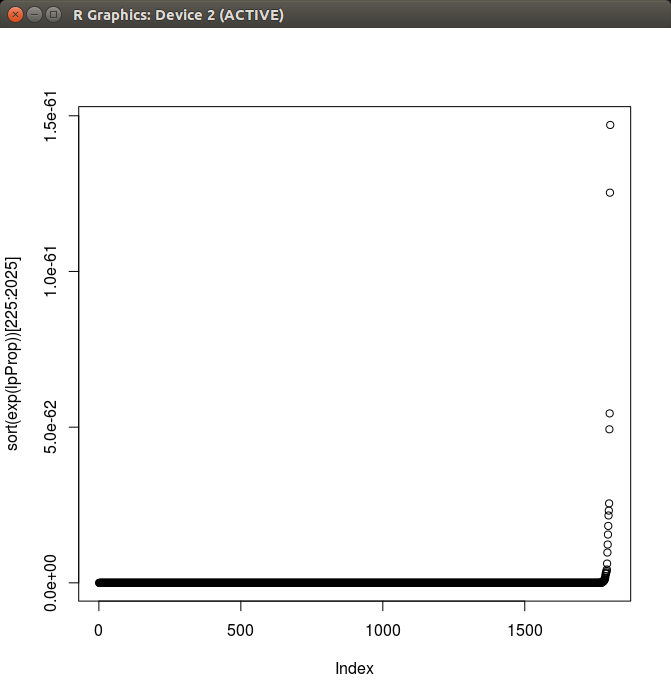
\includegraphics[width=\textwidth]{data/middle80percent1.png}
%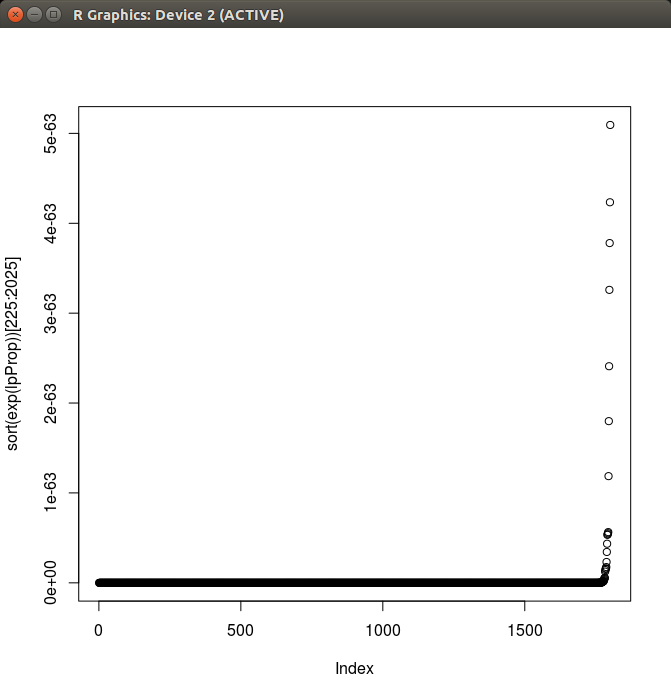
\includegraphics[width=\textwidth]{data/middle80percent2.png}

Below is the information on a log scale. Note that while the probabilities were initially also on a log scale, they have been exponentiated. Also, note that the information doesn't actually follow any kind of a trend. I sorted the data in order to take off the top and bottom 10\%.

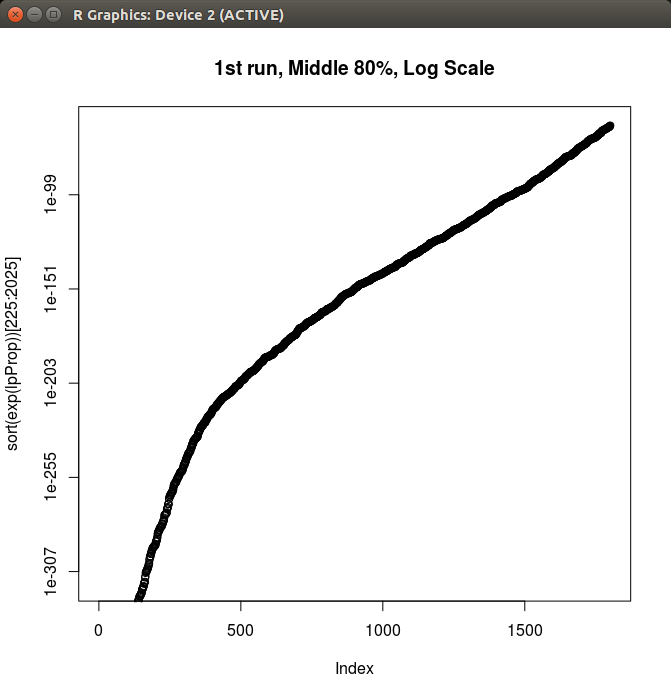
\includegraphics[width=0.5\textwidth]{data/middle80log1.png}
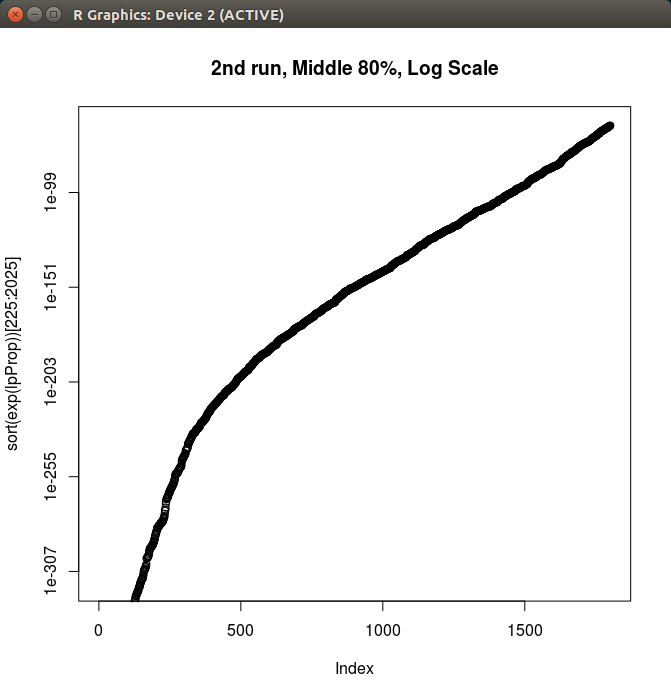
\includegraphics[width=0.5\textwidth]{data/middle80log2.png}

Unfortunately that's all the information I was able to get because the terminal crashed. 

Rerunning using GDB on R. When I hit the browser (when lpProp has NaN), I should be able to launch the C code using GDB and find EXACTLY the error.

\end{enumerate}







\subsubsection{Ideally, an NSE patch to fix it (try NaN to NA?)}

\subsubsection{Disect NSE Data Structure}

Position information? is in reu13.df\$(amino acid)\$Pos

\subsubsection{Rstudio / R vim extension?}

\subsubsection{Reread Debugging Chapter}

Read the section on GDB. Trace seems flexible but not horribly useful in my case.

How to GDB an R session

\begin{enumerate}
\item cd /home/lbrown/cubfits/misc/R\\
\item R -d gdb\\
GDB will launch
\item run\\
(R will run)
\item source("debug\_nsef.r")\\
NSE model will begin in the R session. Run until the R browser catches an error
\item Ctrl-C\\
This returns to GDB (R is still active, but not running).Set a breakpoint.
\item continue\\
R continues running with GDB breakpoint. Launch the code you want to analyze with GDB (and possibly browser)
\end{enumerate}




\subsection{Goals for next Week}
\begin{enumerate}
\item Find out what causes some of the probabilties are going outrageously high
\item If possible, NSE Patch
\item More information on Codon Position
\item Look into an R Vim extension or RStudio
\item (Optional) Find out what trace() does
\end{enumerate}


\section{Week of September 29th - October 1st}
\subsection{Goals for the Week}
%Paste output from writeGoals
\begin{enumerate}
\item What I know from Last Week (kept here for ease of access)
\item Find out what causes some of the probabilties to go outrageously high
\item Compare Min, Max, and Average Values
\item Use Sections of the Simulated Yeast Genome
\item If possible, NSE Patch
\item More information on Codon Position
\item Look into an R Vim extension or RStudio
\item Debugging Thoughts
\end{enumerate}

\subsection{Progress/Notes}

\subsubsection{What I know from Last Week (kept here for ease of access)}

Here's what I know about the NaN error

\begin{enumerate}
\item \sout{one} One or more of the elements of lpProp is going to NaN.
\item It is not always the same element. For my first run, it was zraS. The second was ecnA.
\item It is not because log(0)$= -\infty$. Multiple elements are going to -Inf (106 in the first run,  87 in the second run). Moreover, the roc code also tends to generate -Inf values (though not nearly as many in each run, only 1 or 2).
\item It doesn't appear that the scale is going out of control. Scale and acceptance rate stay similar to the values used in the ROC model.
\item It happens in cubfits and cubappr
\item It is not just happening for one amino acid. For the first run, it happened in Amino Acid 5 (F). In the run, it happened in both 8 and 9 (I and K). The third run happened in 11 (N). In the fourth run, it happened in 3 and 8 (D and I). In the fifth, it was 4 (E).
\item It is lp.vec, the return from my.inverse.mlogit.r
\item my.inverse.mlogit passes NON NaN values (though they are stupidly large like 1.452498e+18 instead of -0.5610390) to invmlogit, and it returns NaN values.
\item The code gets stuck in the following loop

\verbatiminput{misc/stuckHUGE_VALUEloop.txt}

That's what causes the slow down.

But this means the problem comes earlier. At some point in the code, some probabilities are going to infinity, which causes the HUGE\_VALUE loop (and the slowdown), and eventually causes NaN values.

Cedric suggested that it may be caused by the covariance matrix exploding.

\item \sout{All the values} The average values for lpProp are generally too low.\\
mean(lpProp[is.finite(lpProp)]) returns -588.3597 in from the first run, and -554.7103 in the second run.

\item The C code sometimes FIXES the problem! When doing a second run with seed 83455, lp.vec has a NaN value at position 22893 (amino acid???) 

\item The Phi values for codons with -Inf log probability are absurdly high.

\verbatiminput{data/sep29.infPhi.txt}


\end{enumerate}


\subsubsection{Find out what causes some of the probabilties to go outrageously high}

Theories:

One value is going to infinity, for its own reasons. This causes the other values to drop in response, which explains the drop in the average lpProp values. Through some means (addition of the bias? Seems unlikely, logdmultinomCodAllR returns NaN values before the bias comes into effect), I think one of the probabilities goes above 1. Then the odds ratio $\frac{p_{\vec{c}_{ij}}}{1 - p_{\vec{c}_{ij}}} > 1$, which causes the probabilites to EXPLODE. But, it stays under a cap, because stable\_exp.c has the HUGE\_VALUE loop (included above) that keeps things "under control". In attempting to scale the probabilities, it just slows down the code (because it's trying to scale down exponential growth by halves). Eventually, the value becomes so high that the C code cannot process it and returns NaN, which the R code refuses to use for the acceptance vector, and the code crashes.

Alternately, the other values could be going to 0, which causes certain values to become certain (or beyond certain) in response, as opposed to the converse. 

To test this theory, I ran one crash test run of the NSE code (documented), with random seed 83455 and got a NaN number for lp.vec at amino acid 4, in lp.vec[7472]. I'm now rerunning the code with that random seed, and tracking the values of lp.vec[7472]. If I'm correct, it should eventually reach above 0(log probability $> 0$ means probability is $> 1$), and then skyrocket from there.

One other possibility is that it's some kind of numerical error e.g. underflow, and the value lp.vec[7472] will suddenly jump from $-30$ish to $1\times10^{18}$

Results of test: Inconclusive

Setting the random seed to the same value generated DIFFERENT results. Cedric suggests that the MCMC may behave on a separate random seed. This is problematic.


\subsubsection{Compare Min, Max, and Average Values}

grep (min/max/avg/NaN/inf) (file) $\vert$ sort $\vert$ (head/tail)

Wrote a small script, topbot.sh (min/max/avg/NaN/inf) (file)

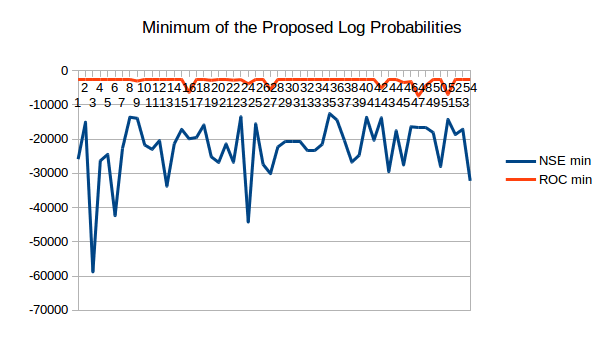
\includegraphics{data/minROCvNSE.png}
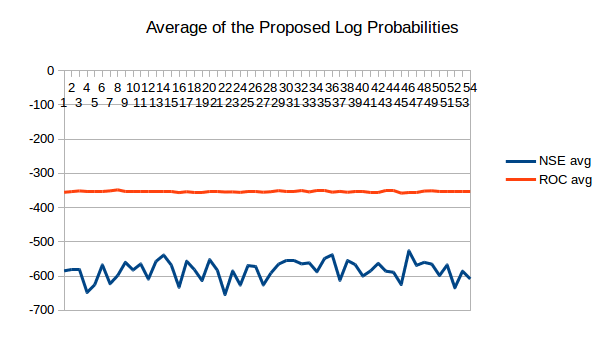
\includegraphics{data/avgROCvNSE.png}
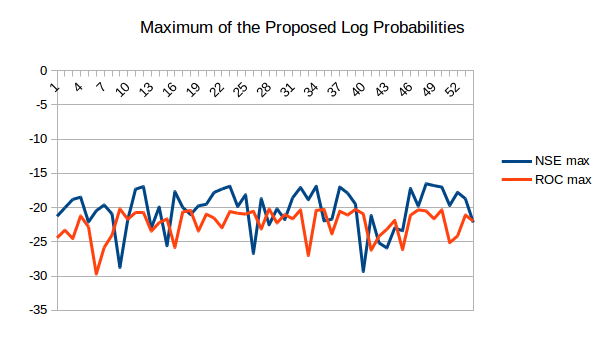
\includegraphics{data/maxROCvNSE.png}

\subsubsection{Use Sections of the Simulated Yeast Genome}

See cubfits/misc/S.cervisiae.REU13/random5ths.r


\subsubsection{If possible, NSE Patch}

One option to look into is to drop lp\_c\_raw from the code, and use rowsums like the Roc model. The two problems with that are that, as far as I can tell, lp.c.raw actually fixes the error in some cases, and using yaa * lp.vec complains for the NSE code. Not sure.

\subsubsection{Look into an R Vim extension or RStudio}

RStudio installed (also CMake), and it's VERY nice. Very intuitive, good use of screen real estate, and it holds a lot of information that I need at once. It keeps launching into /home/lbrown/PACKAGES/rstudio/bin though.

\subsubsection{Debugging Thoughts}

This was in last weeks summary, but it's included here for completeness.

How to GDB an R session
\begin{enumerate}
\item cd /home/lbrown/cubfits/misc/R
\item R -d gdb
\item run
\item source("debug\_nsef.r")
\item Ctrl-C
\item continue
\end{enumerate}



\subsection{Goals for next Week}
\begin{enumerate}
\item NSE Run Sections of Simulated Yeast Geome
\item Find out what causes some of the probabilties to go outrageously high
\item Compare Min, Max, and Average Values
\item Use Sections of the Simulated Yeast Genome
\item Look into an R Vim extension or RStudio
\item Debugging Thoughts
\end{enumerate}


\end{document} 
